% set font size to 12pt, on A4 paper.
\documentclass[12pt]{report}
\usepackage{setspace}
\usepackage[utf8]{inputenc}
\usepackage[a4paper,width=150mm,top=25mm,bottom=25mm,bindingoffset=6mm]{geometry}
\usepackage{booktabs}
\usepackage{graphicx}
\usepackage{amsmath}
\usepackage{subcaption}
\usepackage{fancyhdr}

\usepackage[bookmarks=true,pdftex]{hyperref}
\usepackage{bookmark}
\makeatletter
\AtBeginDocument{
  \hypersetup{
    pdftitle = {\@title},
    pdfauthor = {\@author}
  }
}
\makeatother

\graphicspath{ {images/} }
\setlength{\parskip}{\baselineskip}%
\setlength{\parindent}{0pt}%

\title{Final Year Project Report}
\author{Yash Diniz and Alston Dias and Pranav Paranjape and Rey Dias and Imamsab Bagwan}
\date{2021}

% perform the 1.5 line-spacing for the entire document
\spacing{1.5}


\begin{document}
% \maketitle
% begin page numbering before chapters as roman numerals
\pagenumbering{roman}
% \begin{titlepage}
    \begin{center}
        \Large
        \textbf{DON BOSCO COLLEGE OF ENGINEERING}\\
        \textbf{FATORDA, MARGAO, GOA-403602}

        \normalsize
        \textbf{DEPARTMENT OF COMPUTER ENGINEERING}\\

        \vfill
        
        \large
        \textbf{2020-2021}
        
        
\includegraphics[width=5cm]{logo.jpeg}

        \textbf{“FOCUSA: a comprehensive, scalable,\\
        and real-time e-Learning software”}

        \textbf{By}

        \normalsize
        \textbf{\underline{Mr Yash Diniz}}\\
        \textbf{\underline{Mr Alston Dias}}\\
        \textbf{\underline{Mr Pranav Paranjape}}\\
        \textbf{\underline{Mr Imamsab Bagwan}}\\
        \textbf{\underline{Mr Rey Dias}}\\

        \vfill
        
        Under the guidance of\\
        \textbf{Ms. Maria Christina Barretto}\\
        \textbf{Assistant Professor}\\

        \vfill

        \textbf{Dr. Vivek Jog}\\
        \textbf{Assistant Professor}

    \end{center}
    
\end{titlepage}
%\begin{titlepage}
    \begin{center}
        \begin{tabular}{|c|}
            \hline
                \Large
                BACHELOR OF ENGINEERING: GOA UNIVERSITY\\
            \hline
        \end{tabular}

        \Large
        \textbf{DON BOSCO COLLEGE OF ENGINEERING}\\
        \textbf{FATORDA, MARGAO, GOA-403602}

        \normalsize
        \textbf{DEPARTMENT OF COMPUTER ENGINEERING}\\

        \vspace*{0.4cm}
        
        \large
        \textbf{2020-2021}
        
        
\includegraphics{logo.jpeg}

    \end{center}
\end{titlepage}
\chapter*{ABSTRACT}

Colleges, schools and other educational environments have a lot of existing tools which help students and teachers interact and share resources. 
These tools, however, are developed to serve very specific and limited purposes and are very difficult to manage manually. 
Most of them fail to provide a single comprehensive platform for all necessary management operations. 
Moreover, these existing tools also fail to cater to the management and analysis of data and thus are not used for generating insights and management optimisation.

Our project aims to deliver a scalable web services framework which is easy to work with for both the developer and the customers. 
It will allow connecting students and teachers through subscription portals, by letting faculty moderators post content which can be accessed by the students and synced whenever an internet connection is available. 
Furthermore, we aim to build a real-time video conferencing platform using a lossy compression algorithm involving neural networks. 
Finally, we plan on integrating various existing services like Google Calendar and Drive, to ease automation efforts, reducing the need to manually manage multiple tools.

\chapter*{ACKNOWLEDGMENT}

First and foremost, we would like to thank the Director \textbf{Fr. Kinley D’ Cruz}, 
Principal \textbf{Dr. Neena S. P. Panandikar} and Head of Department \textbf{Dr. Gaurang Patkar} 
for providing all the help we needed.

The team put in a lot of effort on the project. However, it would not have 
been possible to complete it without the help of the faculty.

We are highly indebted to \textbf{Miss Maria Christina Barretto} for her guidance 
and constant supervision as well as for providing necessary information 
regarding the project and to our co-guides \textbf{Dr. Vivek Jog} and \textbf{Miss Nisha 
Godhino} for their guidance.

We would like to take this opportunity to thank the institution 
\textbf{DON BOSCO COLLEGE OF ENGINEERING} and the faculty members of the 
Computer Engineering Department who helped and supported us to 
go ahead with the project.


\tableofcontents
\pdfbookmark{\contentsname}{Contents} % add a bookmark to Table of contents
\listoffigures
% \listoftables

\chapter{Introduction}

% restarting page numbering from Introduction as stated in project report guidelines.
\pagenumbering{arabic}

The essence of education is the ability for teachers to efficiently 
disseminate knowledge and obtain positive feedback from students, by 
using tools for a good teaching-learning experience. 
Educational environments have a lot of existing tools which help students 
and teachers interact and share resources. These tools, as will be explained 
further in this report, are developed to serve very specific and limited 
purposes, and are difficult to manage manually. They fail to provide a 
single comprehensive platform for all necessary operations. 
Moreover, these existing tools fail to cater to the management and analysis 
of data and thus are not used for generating insights and management optimisation. 
Furthermore, our worldwide internet infrastructure is lacking the reliability it 
needs to help people stay connected~\cite{WebF20}.

\section{Problem Definition}

Multiple e-learning platforms exist, each trying to solve a unique problem. 
Very few platforms function using an offline-first architecture, thus leading to 
really high dependency on network infrastructure. 
It gets difficult for both students and teachers to manage their work, 
since they have to use multiple platforms, dividing their attention among each of them. 
Current e-learning platforms also provide very little in the way of automation, 
and lack a common, integrable interface.

Not all software platforms are built considering unreliable internet service. 
This dependency on a reliable internet by a majority of its users thus affects the entire network, 
and reduces quality of service for all internet users.This problem can be solved in many ways, 
like improving the network infrastructure, or building applications that 
responsibly use internet bandwidth. If unattended, issues of an unreliable 
system can include lesser productivity.

\subsection{Existing Systems}

There are a lot of e-learning systems and platforms available in the market 
but the most popular ones are Google Classroom and Moodle. 
The following shall be a brief overview of these popular e-learning platforms.

\subsubsection{Google Classroom}
% Pranav Paranjape
To quite an extent google classroom managed to replace the traditional 
learning management system with no paper requirement, easy document sharing using google docs, 
easy assignment submission process and features to integrate with other Google services 
like YouTube, Drive and even Meet. 
We feel it still couldn’t fully become the replacement for education system because of the following:

\begin{itemize}
    \item \textbf{Difficult account management.} Suppose the user wants to upload an assignment onto the classroom for submission, 
    which is currently on another google account, the user will need to logout of the current account, 
    download the document and sign in with the required Google account and upload; quite a hassle.
    \item \textbf{Doesn’t have an offline first design}, which eliminates the need of always being online to access the documents, 
    as the documents can be downloaded in the user’s local storage for a limited amount of time.
    \item \textbf{No live post updates}, i.e. the user need to keep refreshing to view the recent updates.
\end{itemize}

One biggest pros of google education services is modularity. The G-Suite offers all these 
loosely coupled services like Meet, Classroom, Hangouts, and many others.

\subsubsection{Moodle}
% Pranav Paranjape
Yet another popular e-learning platform and the best alternative to Google Classroom. 
Its pros include limited offline use for certain features. It has impressive features 
for  uploading and downloading lecture notes, creating quizzes and tests, supports push 
notifications for both students and teachers, generating reports and many others. 
It has a  backup, restore and import features, which turn out to be really useful for teachers. 
The teachers can also manage learners' profiles and setting enrollment keys, with role-based restrictions.

One of it’s biggest cons however include poor scalability, due to its tightly coupled nature. 
This also causes issues with robustness, since a single module crash can cause the whole system to crash. 
No inbuilt video-conferencing functionalities, and it also becomes difficult to integrate a 
third party service due to the same tightly coupled nature.

It also offers a relatively poor mobile offering, with limited integration into third-party modules. 
There is a major learning curve for building and taking Moodle administration courses for beginners.

\subsubsection{Active Document Platform}
% Yash Diniz
The Active Document Platform(AD)~\cite{ActiveDocument} is a very useful platform that 
solves the problem of unreliable internet connectivity, by serving as an offline-first 
and distributed way of sharing course documents. Not being dependent on a centralised 
server on the internet allows it to operate offline as well, and it synchronizes with 
its main node whenever internet connectivity gets established. The best part about AD 
is its document organization, and distributed collaborative editing. Furthermore, AD 
uses SCORM (Sharable Content Object Reference Model), which is a collection of standards 
and APIs which help streamline connecting between other e-learning platforms which also 
use SCORM. One of its biggest cons however is limited functionality, and not very user-friendly.

\subsection{Proposed System}

Our project aims to deliver a scalable web services framework which is easy to work with 
for both the developer and the customers. It will allow connecting students and teachers 
through subscription portals, by letting faculty moderators post content which can be accessed 
by the students and synced whenever an internet connection is available. 
Furthermore, we aim to build a real-time video conferencing platform using a lossy compression 
algorithm involving neural networks. 
Finally, we plan on integrating various existing services like Google Calendar and Drive, 
to ease automation efforts, reducing the need to manually manage multiple tools.

\section{Purpose of the Project}

We plan on integrating various existing services so that the students need to use a single application interface, 
and are kept updated. We will work towards reducing network bandwidth usage, adopting an offline-first architecture 
wherever applicable. 
We will also add many optimizations, especially in video conferencing by intelligently encoding only the 
required features and intelligently transmitting it. We will also build interfaces to anonymously collect and 
analyze data which can be used to measure, manage various processes by finding out patterns that can help teachers 
improve their course material, and allowing us to focus on what matters, letting the computer automate various 
basic operations for us. We will also work to make our project scalable, robust, and flexible, allowing integrations 
to various third-party modules using our API.

\section{Scope of the Project}
% Alston Dias
\subsubsection{Must be implemented}
\begin{itemize}
    \item Scalable and loosely coupled Web Services Framework.
    \item Connecting students and teachers through subscription portals (courses), 
    which can be made private by virtue of an authentication code if needed.
    \item Allowing faculty and students to have specific roles, which are moderated by limited people.
\end{itemize}

\subsubsection{Should be implemented}
\begin{itemize}
    \item Integrating various existing services, like Google Calendar, Drive, classroom, etc. 
    by building web-hooks, which allow for easy automation. (by virtue of bots)
    \item A real-time video conferencing platform using an experimental lossy compression algorithm involving neural networks.
\end{itemize}

\subsubsection{Could be implemented}
\begin{itemize}
    \item Having a marketplace for modules, where it is as easy as integrating by pressing install.
    \item Creating a simple student planner application that can help the student manage submissions, 
    projects, and time in general (integrated with Calendar for ease of use)
    \item A system that can perform collection, monitoring, reporting, and long-term benefit analysis 
    of student and employee attendance at the college. It can help students set their priorities.
    \item An online test tool that allows faculty to create tests and students can answer tests.
\end{itemize}

\section{Report Organization}

The current introductory section provides a brief introduction to each chapter.

\textbf{Chapter 1: Introduction}

This section focuses on the purpose and scope of the proposed system of FOCUSA.

\textbf{Chapter 2: Literature Survey}

This section describes the concepts and technologies used to develop the project.

\textbf{Chapter 3: Software Requirement Specification}

This section provides information about the specific requirement of the proposed system.

\textbf{Chapter 4: Design}

This section describes the software lifecycle model, which will be used in developing the
software. It also includes system design and detailed design.

\textbf{Chapter 5: Implementation}

This section deals with the implementation of the project where in the snapshots of each execution steps are shown.

\textbf{Chapter 6: Conclusion}

This section deals with the conclusion that can be derived after implementing the final System.

\chapter{Literature Survey}

\section{WebRTC}

WebRTC (Web Real-Time Communication) is a free, open-source project providing web browsers and 
mobile applications with real-time communication via simple Application Programming Interfaces (APIs). 
It allows audio and video communication to work inside web pages by allowing direct peer-to-peer 
communication, eliminating the need to install plugins or download native apps.
It supports video, voice, and generic data to be sent between peers, allowing developers 
to build powerful voice- and video-communication solutions.~\cite{wikiWebRTC}

There are 3 primary components of the WebRTC API and each plays a unique role in WebRTC specification:

\subsubsection{MediaStream (GetUserMedia)}

The MediaStream API provides a way to access device cameras and microphones using JavaScript. 
It controls where multimedia stream data is consumed, and provides some control over the devices 
that produce the media. It also exposes information about devices able to capture and render media.

\subsubsection{RTCPeerConnection}

The Peer Connection is the core of the WebRTC standard. It provides a way for participants to 
create direct connections with their peers without the need for an intermediary 
server (beyond signalling). Each participant takes the media acquired from the media 
stream API and plugs it into the peer connection to create an audio or video feed.  
The PeerConnection API has a lot going on behind the scenes. It handles SDP negotiation, 
codec implementations, NAT Traversal, packet loss, bandwidth management, and media transfer.

\subsection{RTCDataChannel}

The RTCDataChannel API was setup to allow bi-directional data transfer of any 
type of data - media or otherwise - directly between peers. It was designed to mimic the 
WebSocket API, but rather than relying on a TCP connection which although reliable is high 
in latency and prone to bottlenecks, data channels use UDP-based streams with the configurability 
of the Stream Control Transmission Protocol (SCTP) protocol. This design allows the best 
of both worlds: reliable delivery like in TCP but with reduced congestion on the network like in UDP.

\subsection{Establishing the connection}

Before a peer-to-peer video call can begin, a connection between the two clients 
needs to be established. This is accomplished through signalling. Signalling falls 
outside of the realm of the WebRTC specification but is the vital first step in establishing 
an audio/video connection.

\subsection{Signalling}

Signalling allows two endpoints (senders, receivers, or both) to exchange metadata to 
coordinate communication in order to set up a call. This call-and-response message flow 
contains critical details about the streaming that will take place, that is, the number 
and types of streams, how the media will be encoded, etc. 

This is needed for two reasons: because the communicating peers do not know each other’s 
capabilities, and the peers do not know each other’s network addresses.

\subsection{NAT Traversal - ICE, TURN and STUN}

Once the initial signalling for a streaming connection has taken place, the two endpoints need 
to begin the process of NAT (Network Address Translation) traversal.
This assigns a public address to a computer inside a private network for setting up a real-time connection. 
In a WebRTC-enabled communication, unless the two endpoints are on the same local network, 
there will be one or more intermediary network devices (routers/gateways) between the two. 
There are three key specifications that are used in WebRTC to overcome these hurdles:

\begin{itemize}
    \item \textbf{Interactive Connectivity Establishment (ICE)} - ICE is used to find all the ways 
    for two computers to “talk to each other”. It has two main roles, gathering candidates 
    and checking connectivity. It guarantees that if there is a path for two clients to communicate, 
    it will find it and ensure it is the most efficient. It makes use of two protocols - STUN and TURN.
    \item  \textbf{Session Traversal Utilities for NAT (STUN)}  – It is a lightweight and simple 
    method for NAT Traversal. STUN allows WebRTC clients to find out their own public IP address 
    by making a request to a STUN server. 
    \item  \textbf{Traversal Using Relays around NAT (TURN) }  - The TURN server assists in the NAT 
    traversal by helping the endpoints learn about the routers on their local networks, 
    as well as blindly relaying data for one of the endpoints where a direct connection is 
    not possible due to firewall restrictions.
\end{itemize}

\begin{figure}
\begin{center}
    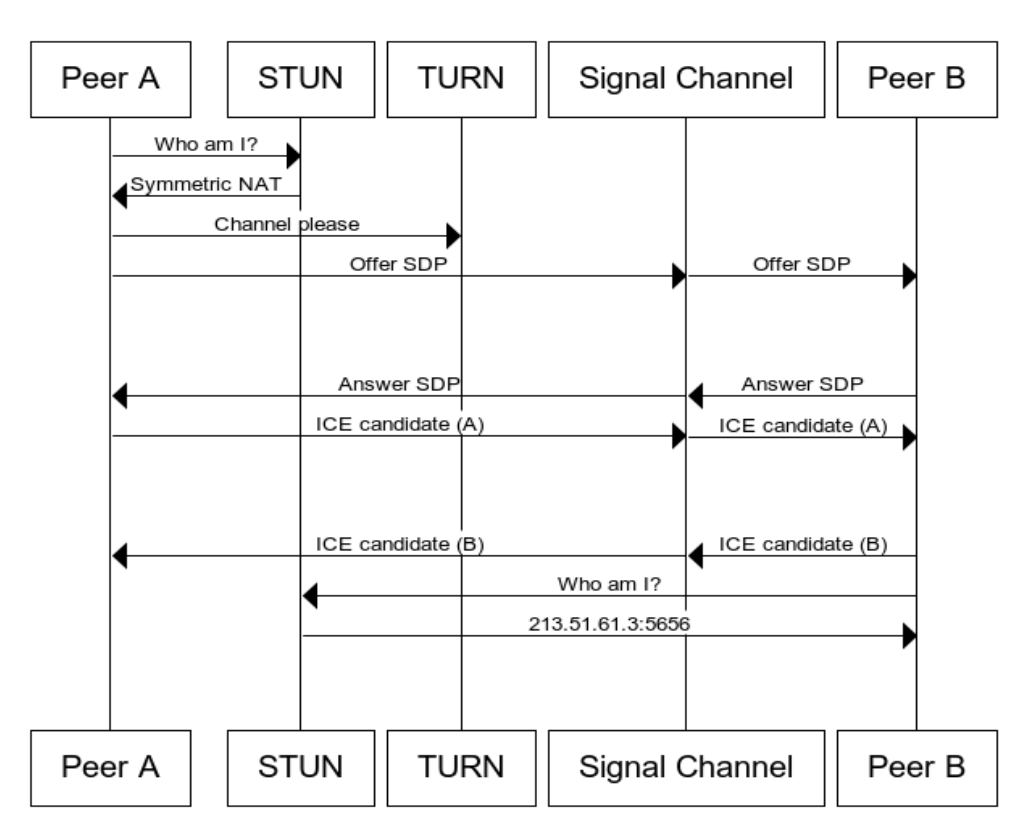
\includegraphics[width=10cm]{webRTC.png}
\end{center}
\caption{Call Service: webRTC Signalling Plane}
\label{fig:webrtc}
\end{figure}

\subsection{Codecs}

Before sending the media over a peer connection, it has to be compressed. 
Raw audio and video is simply too large to send efficiently in our current Internet infrastructure.
Likewise, after receiving media over a peer connection, it has to be decompressed. 
For this, use a media codec.

WebRTC has mandated three audio codecs and two video codecs:

\begin{enumerate}
    \item Audio - PCMU (G.711$\mu$) running at 8,000Hz with a single channel (mono).
    \item Audio - PCMA (G.711a) running at 8,000Hz with a single channel (mono).
    \item Audio - Opus running at 48,000Hz with two channels (stereo).
    \item Video - VP8.
    \item Video - H.264/AVC using Constrained Baseline Profile Level 1.2.
\end{enumerate} 

The technology is available on all modern browsers as well as on native clients for
all major platforms. The technologies behind WebRTC are implemented as an open web 
standard and available as regular JavaScript APIs in all major browsers. For native clients, 
like Android and iOS applications, a library is available that provides the same 
functionality.~\cite{UltimateGuideWebRTC}

\section{MATRIX}

Matrix is an open protocol for decentralised communication. It aims to make 
communication platforms interoperable and federated.

The main idea is to make real-time communication work seamlessly between different chat 
service providers, allowing users with accounts at one communications service provider to 
easily communicate with users of a different service provider.

Users have the privilege to communicate with people outside the Matrix network through bridges, 
which connect previously established communication networks, such as Slack and IRC, to the Matrix network.
With bridges, you do not have to use different apps to talk to different people. Whatever Matrix 
client you choose, you can talk to anyone inside or outside the Matrix network.

Matrix gives users total control over their communication by letting them run or select their own 
server while still participating in a global network, rather than being locked in silos 
like Signal, WhatsApp, Telegram, Slack etc. 

The key feature of Matrix is that no single server hosts or controls a given conversation - instead, 
as one user communicates with another, the conversation gets replicated equally across the servers - meaning 
all the participants equally share ownership over the conversation and its history. 
There is never a central point of control or authority, 
unless everyone decides to use the same server.~\cite{MATRIXorgOpenProtocol}

By default, Matrix uses simple HTTPS+JSON APIs as its baseline transport, but also embraces 
more sophisticated transports such as WebSockets or ultra-low bandwidth Matric via CoAP+Noise.~\cite{MATRIX}

Applications using the Matrix protocol, called Matrix clients, have all the features one would
want and expect from a modern chat app: instant messaging, group chats, audio and video calls, 
searchable message history, synchronization across all devices, as well as end to end encryption.
Element is the best known Matrix client.
Via Matrix, Element is able to bridge communications like IRC, Slack and Telegram into the app.~\cite{RumaMATRIX}

\begin{figure}[h]
    \begin{center}
        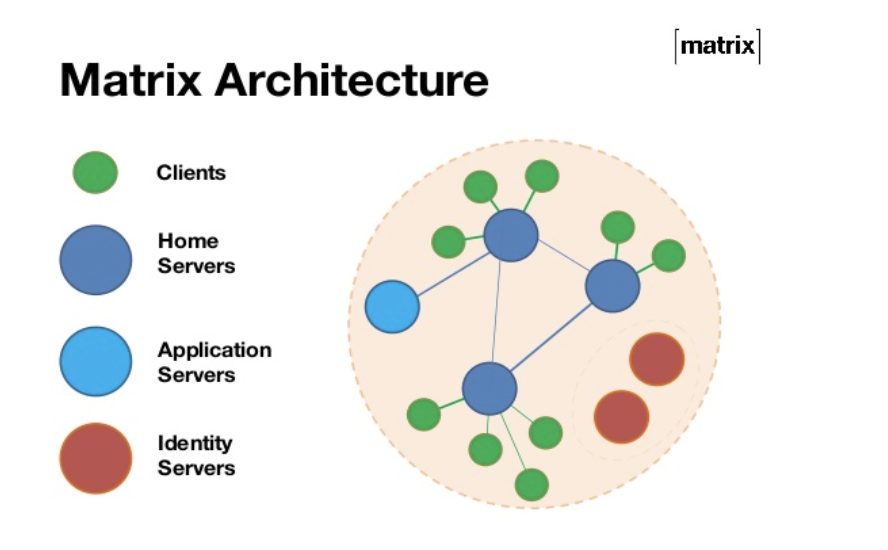
\includegraphics[width=10cm]{matrix.png}
    \end{center}
    \caption{An example of a Matrix Architecture, illustrated very simply using abstract coloring.}
    \label{fig:matrix}
\end{figure}

\subsection{Why MATRIX?}

As a result of several chat services not being interoperable with each other, people are 
forced to use multiple services to communicate.
However, since Matrix is federated, just like email, you can freely communicate across a 
global network, without having to use specific services based on which ones your friends, 
family, and colleagues use.

Another major problem with online communication today is that most of the services you
use are operated by commercial organizations, forcing you to trust them to manage your data.
But because Matrix is federated, you have control over where your data is stored and who has access to it.~\cite{RumaWhyMatrix} 

\section{PeerJS}

The PeerJS library is aimed to simplify the peer-to-peer connection management. 
PeerJS wraps the browser's WebRTC implementation to provide a complete, configurable, 
and easy-to-use peer-to-peer connection API. 
With PeerJS, peers are identified by simply using an ID, a string that the peer 
can choose itself, or have a server generate one. 
Equipped with an ID, a peer can create a P2P data or media stream connection to a remote peer.~\cite{PeerJSsimplifiesWebRTC}

\subsection{PeerJS Server}

Although WebRTC promises peer-to-peer communication, a server is still required to 
act as a connection broker, and handle signalling.

PeerJS provides an open source implementation of this connection broker 
server named PeerJS Server, written in Node.js.Users can run their own Server, 
or are at leisure to opt for the cloud-hosted version of PeerServer provided for free.
To broker connections, PeerJS connects to a PeerServer. The PeerJS Server acts ONLY as 
a connection broker, and it has to be noted that no peer-to-peer data goes through the server.~\cite{TamingWebRTCwithPeerJS}

To make the P2P connection work seamlessly, we will build the neural network encoder and 
integrate it into WebRTC possibly using the P2P library.

\section{REST API}

A REST API is an application programming interface that conforms to the constraints of the REST 
architectural style and allows for interaction with RESTful web services.

REST is not a standard, but rather a set of recommendations and constraints for 
RESTful web services. These include:

\begin{enumerate}
    \item \textbf{Client-Server.} System ‘A’ makes an HTTP request to a URL hosted by 
    System ‘B’, which returns a response.
    It is identical to how a browser works: The application first makes a request 
    for a specific URL, the request is then routed to a web server that returns an HTML page. 
    This page may contain references to images, style sheets, and JavaScript, 
    which incur further requests and responses.

    \item \textbf{Stateless.} REST is stateless: the client request should contain all the 
    information necessary to respond to a request. In other words, it should be possible to
    make two or more HTTP requests in any order and the same responses will be received.

    \item \textbf{Cacheable.} A response should be defined as cacheable or not.
    
    \item \textbf{Layered.} The requesting client need not know whether it’s communicating 
    with the actual server, a proxy, or any other intermediary.~\cite{DevelopersRestAPI}
\end{enumerate}

The working first involves sending a request from the client to the server in the form of web URLs, 
using the HTTP GET, POST, PUT or DELETE methods. After that a response is retrieved from the server 
in the form of a resource which can be anything like HTML, XML, Image or JSON.~\cite{WhatisRESTAPI}

\begin{figure}
    \begin{center}
        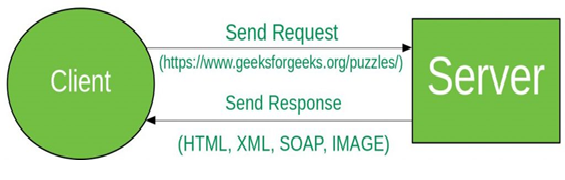
\includegraphics[width=8cm]{restapi.png}
    \end{center}
    \caption{A simple illustration of a REST API request-response.}
    \label{fig:restapi}
\end{figure}

In HTTP there are five methods which are commonly used in a REST based Architecture 
i.e. POST, GET, PUT, PATCH, and DELETE. These methods correspond to create, read, 
update, and delete (or CRUD) operations respectively.~\cite{GeeksRestAPI}

\section{GraphQL}

GraphQL is a query language and server-side runtime for Application Programming Interfaces (APIs) 
that prioritizes giving clients exactly the data they request and nothing more. 
GraphQL is designed to make APIs fast, flexible, and developer-friendly. It is not tied 
to any specific database or storage engine and is instead backed by your existing code and data.

API developers use GraphQL to create a schema to describe all the possible data that clients can query 
through that service. This schema is made up of object types, which define which kind of object you can 
request and what fields it has. As queries come in, GraphQL validates the queries against the schema. 
GraphQL then executes the validated queries.

The API developer attaches each field in a schema to a function called a resolver. 
During execution,the resolver is called to produce the value.~\cite{WhatisGraphQL}

GraphQL follows the same set of constraints as REST APIs, but it organizes data into a 
graph using one interface. Objects are represented by nodes (defined using the GraphQL schema), 
and the relationship between nodes is represented by edges in the graph. Each object is then backed 
by a resolver that accesses the server’s data.

When a GraphQL server responds to an end user’s request, it begins with the query root,
and the resolver executes every field on the requested object. A key-value map houses each field’s
values, and some return another object selecting another set of fields. This continues until only a 
string or a number is returned. The server then responds with a nested set of objects, as requested by 
the end user.~\cite{RubrikGraphQL}

\begin{figure}
    \begin{center}
        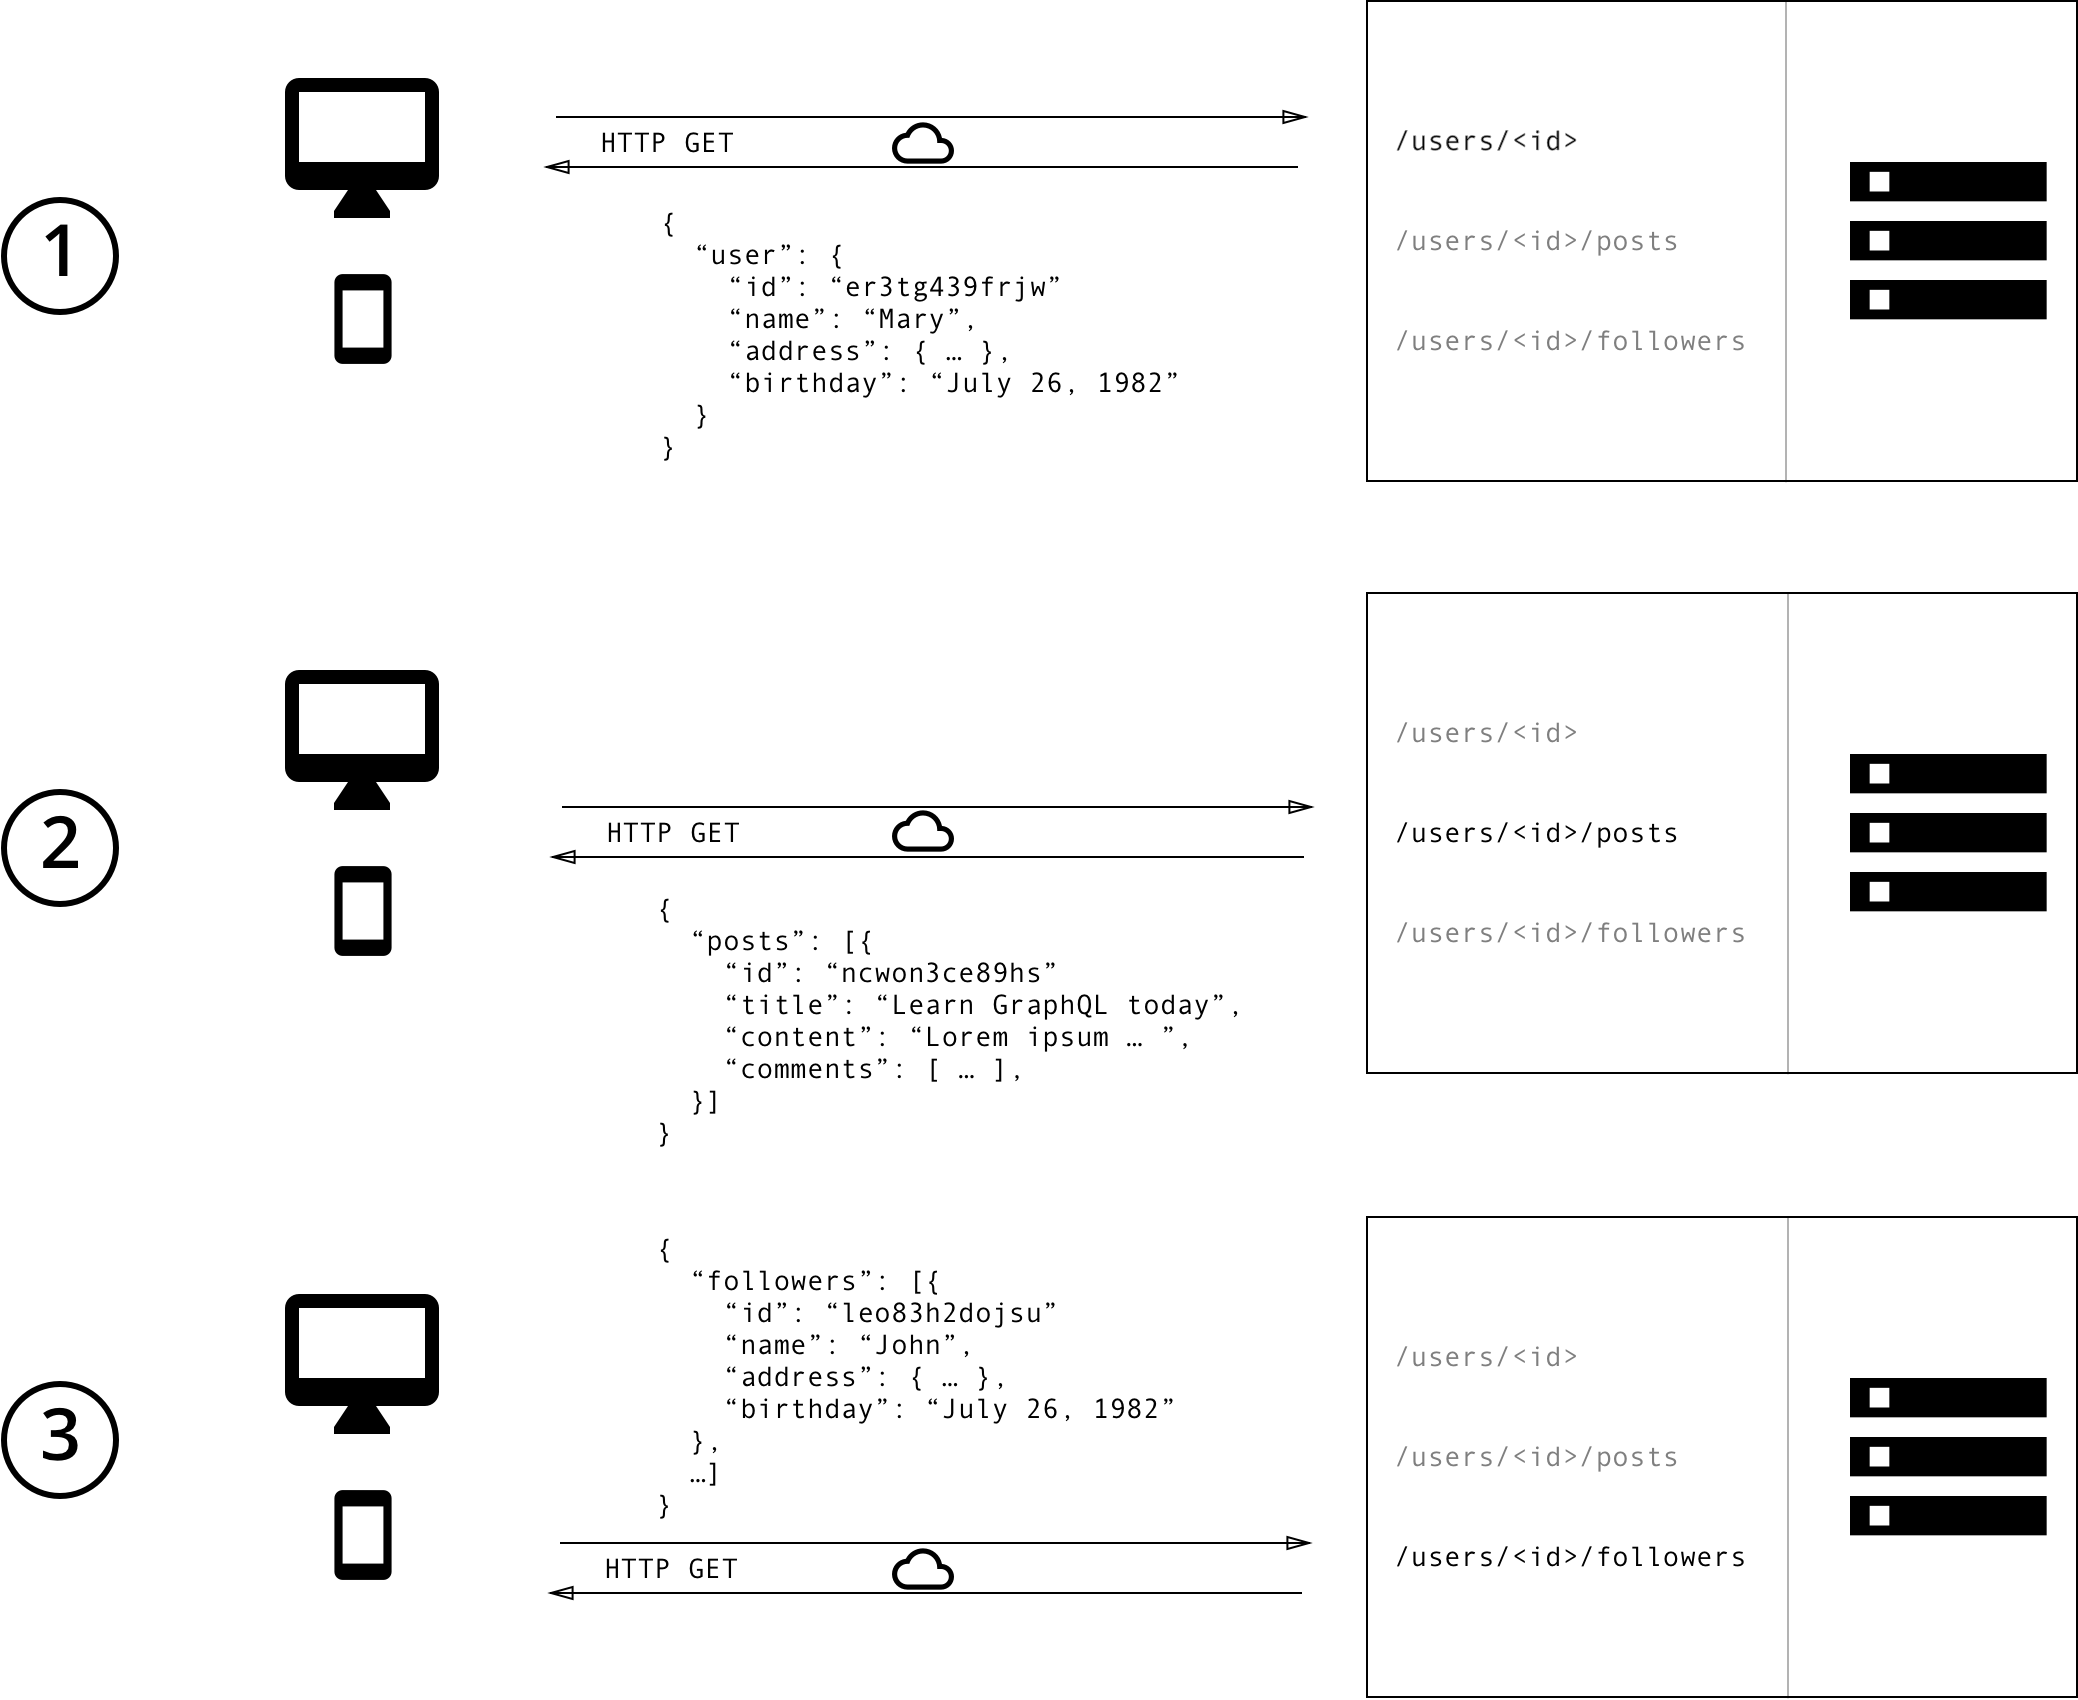
\includegraphics[width=15cm]{graphql-rest.png}
    \end{center}
    \caption{GraphQL can handle the tasks of multiple REST endpoints, 
    neither overfetching, nor underfetching,
    offering the exact data format as requested by the client.}
    \label{fig:graphql}
\end{figure}
  
\subsection{How does GraphQL excel REST API?}

\subsubsection{Data Fetching}

With a REST API, you would typically gather the data by accessing multiple endpoints. You basically 
end up having to make multiple requests to different endpoints to fetch the required data.
In GraphQL on the other hand, you’d simply send a single query to the GraphQL server that 
includes the concrete data requirements. The server then responds with a JSON object where these 
requirements are fulfilled. Therefore using GraphQL, the client can specify exactly the data it needs in a query.

\subsubsection{Over-fetching and Under-fetching of Data}

One of the most common problems with REST is that of over-fetching and under-fetching. This happens 
because the only way for a client to download data is by hitting multiple endpoints that return fixed data structures.
GraphQL gives the clients the exact data they request for.

\subsubsection{Benefits of a Schema and Type System}

GraphQL uses a strong type system to define the capabilities of an API. All the types that are exposed in an API 
are written down in a schema using the GraphQL Schema Definition Language (SDL). This schema serves as the contract 
between the client and the server to define how a client can access the data.
Once the schema is defined, the teams working on frontend and backends can do their work without further communication 
since they both are aware of the definite structure of the data that’s sent over the network.
Frontend teams can easily test their applications by mocking the required data structures. Once the server is ready, 
the switch can be flipped for the client apps to load the data from the actual API.

\subsubsection{Rapid Product Iterations on the Front-end}

A common pattern with REST APIs is to structure the endpoints according to the views that you have inside your app 
in order for the client to get all required information for a particular view by simply accessing the corresponding 
endpoint. However, the major drawback of this approach is that it doesn’t allow for rapid iterations on the frontend. 
With every change that is made to the UI, there is a high risk that now there is more or less data required than before.
Consequently, the backend needs to be adjusted as well to account for the new data needs. This notably slows down the 
ability to incorporate user feedback into a product. But owing to the flexible nature of GraphQL, changes on the 
client-side can be made without any extra work on the server. Since clients can specify their exact data requirements, 
no backend adjustments are required when the design and data needs on the frontend change.

\subsubsection{Insightful Analytics on the Back-end}

GraphQL allows you to have fine-grained insights about the data that’s requested on the backend. As each client specifies 
exactly what information it’s interested in, it is possible to gain a deep understanding of how the available data is being 
used. This can for example help in evolving an API and deprecating specific fields that are not requested by any clients any more.
With GraphQL, you can also do low-level performance monitoring of the requests that are processed by your server. 
GraphQL uses the concept of resolver functions to collect the data that’s requested by a client. Instrumenting and measuring 
performance of these resolvers provides crucial insights about bottlenecks in your system.~\cite{GraphQLvsREST}

\section{NVIDIA Maxine}

We have added NIVIDA MAXINE as a literature survey to share that we are aware of 
a similar service offering video conferencing services using AI. We will take 
inspiration from NVIDIA's technology and attempt to overcome their disadvantages.

NVIDIA Maxine is a fully accelerated platform SDK for developers of video 
conferencing services to build and deploy AI-powered features that use state-of-the-art 
models in their cloud. Video conferencing applications based on Maxine can reduce video 
bandwidth usage down to one-tenth of H.264 using AI video compression, dramatically reducing costs.

Maxine includes APIs for the latest innovations from NVIDIA research such as face alignment, 
gaze correction, face re-lighting and real time translation in addition to capabilities such 
as super-resolution, noise removal, closed captioning and virtual assistants. These capabilities are 
fully accelerated on NVIDIA GPUs to run in real time video streaming applications in the cloud.

Maxine-based applications let service providers offer the same features to every user on any device,
including computers, tablets, and phones. Applications built with Maxine can easily be deployed as 
microservices that scale to hundreds of thousands of streams in a Kubernetes environment.~\cite{Maxine}

\subsection{Features}

\begin{itemize}
    \item \textbf{Easy to use SDK}: Includes libraries, tools and example pipelines 
    for developers to quickly add AI features to their applications.
    \item \textbf{Ultra-low Bandwidth}: AI Video Compression uses one-tenth the 
    bandwidth of H.264 video compression standard.
    \item \textbf{State-of-the-art AI model}: Includes pre-trained models with thousands of hours 
    of training on NVIDIA DGX\texttrademark A100.
    \item \textbf{Fully GPU Accelerated}: Optimizes end-to-end pipelines for the highest performance 
    on NVIDIA Tensor Cores GPUs.
\end{itemize}

\subsection{Key Technologies}

\subsubsection{Reduce Video Bandwidth compared to H.264}
With AI-based video compression technology running on \textbf{NVIDIA GPUs}, 
developers can reduce bandwidth use down to one-tenth of the bandwidth needed 
for the H.264 video compression standard. This cuts costs for providers and 
delivers a smoother video conferencing experience for end users, who can enjoy 
more AI-powered services while streaming less data on their computers, tablets, and phones.

\subsubsection{Face Re-Animation}
Using new AI research, you can identify key facial points of each person on a video call 
and then use these points with a still image to reanimate a person’s face on the other side 
of the call using Generative Adversarial Networks (GANs).

These key points can be used for face alignment, where faces are rotated so that
people appear to be facing each other during a call, as well as gaze correction 
to help simulate eye contact, even if a person’s camera isn’t aligned with their screen.

Developers can also add features that allow call participants to choose their
own avatars that are realistically animated in real time by their voice and emotional tone.

\subsubsection{Video and Audio Effects}
AI-based super-resolution and artifact reduction can convert lower resolutions to higher
resolution videos in real time which helps to lower the bandwidth requirements for video 
conference providers, as well as improves the call experience for users with lower bandwidth. 
Developers can add features to filter out common background noise and frame the camera on a user’s 
face for a more personal and engaging conversation.

Additional AI models can help remove noise from low-light conditions creating a more appealing picture.

\subsubsection{Conversational AI}
Maxine-based applications can use NVIDIA Jarvis, a fully accelerated conversational
AI framework with state-of-the-art models optimized for real time performance. Using Jarvis, 
developers can integrate virtual assistants to take notes, set action items, and answer questions 
in human-like voices.

Additional conversational AI services such as translations, closed captioning and transcriptions help 
ensure everyone can understand what’s being discussed on the call.

\subsection{Disadvantages}

NVIDIA Maxine needs all of its devices to have NVIDIA hardware or access to the NVIDIA cloud. 
This reduces the customer base because of its cost and huge unavailability of GPUs.

It is therefore important to understand that dependence on compute-intensive hardware could
currently be our only barrier to building effective applications using Neural Networks.

\section{Neural Discrete Representation Learning}

Recent advances in generative modelling of images, audio and videos have yielded impressive
samples and applications. At the same time the challenges that follow these tasks are few-shot
learning, domain adaptation, or reinforcement learning heavily rely on learnt representations from raw data.

Learning representations with continuous features have been used in many previous 
work but discrete representations  are potentially more natural fit for many applications. 
Discrete representations are a natural fit for complex reasoning, planning and predictive learning
(e.g., if it rains, I will use an umbrella).

This concept of discrete representation gave rise to the Vector Quantization-Variational Autoencoder. 
This model relies on Vector Quantization with the combination of Variational Autoencoder framework with 
discrete latent representations through a novel parameterisation of the posterior distribution of (discrete) 
latents given an observation.~\cite{oord2018neural}

\subsection{Vector Quantization - Variational Autoencoder (VQ-VAE)}

VAEs consist of the following parts: an encoder network which parameterised a posterior  
distribution $q(z|x)$ of discrete latent random variables $z$ given the input data $x$, a prior
distribution $p(z)$, and a decoder with a distribution $p(x|z)$ over input data.

Typically, the posteriors and priors in VAEs are assumed normally distributed with diagonal 
covariance. Extensions include autoregressive prior and posterior models, normalising flows, 
and inverse autoregressive posteriors . VQ-VAE uses discrete latent variables which is  
a new way of training, by using vector quantisation (VQ). The posterior and prior distributions are 
categorical, and the samples drawn from these distributions index an embedding table. These embeddings
are then used as input into the decoder network.

\subsection{Discrete Latent Variables}

Let's define a latent embedding space $e \in R^{K \times D}$ where $K$ is the size of the discrete latent space 
(i.e., a $K$-way categorical), and $D$ is the dimensionality of each latent embedding vector $e_{i}$.
Note that there are $K$ embedding vectors $e_{i} \in R ^D$, $i\in{1, 2, ..., K}$.

The discrete latent variables $z$ are then calculated by a nearest 
neighbour look-up using the shared embedding space $e$ as shown in equation \ref{eqn:discrete}.

\begin{equation}
q(z = k|x) =
\begin{cases}
    1 & \text{for } k = \text{argmin}_{j} \| z_{e}(x) - e_{j} \|_{2} \\
    0 & \text{otherwise}
\end{cases}
\label{eqn:discrete}
\end{equation} 

where $z _e(x)$ is the output of the encoder network.

The input to the decoder is the corresponding embedding vector $e _k$ as given in equation \ref{eqn:decoder}
\begin{equation}
    z _q(x) = e _k, \text{where } k= \text{argmin} _j \| z _e(x) - e _j \| _2
    \label{eqn:decoder}
\end{equation}

\subsection{Learning}

\begin{figure}[h]
    \begin{center}
        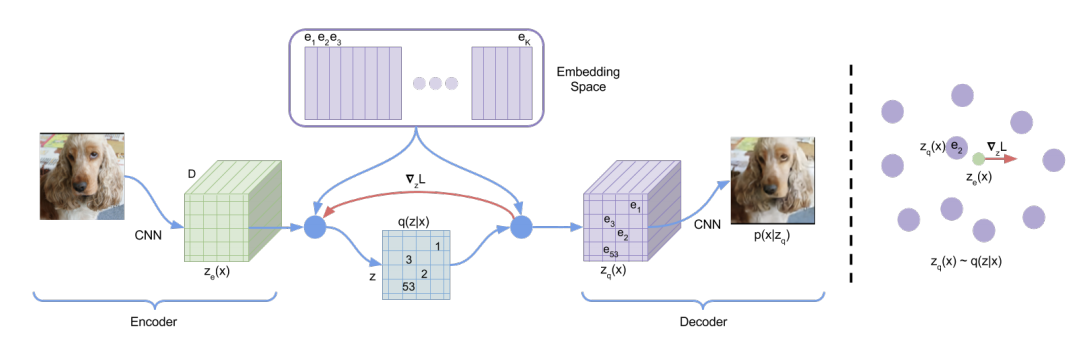
\includegraphics[width=15cm]{vqvae.png}
    \end{center}
    \caption{Left: A figure describing the VQ-VAE. Right: Visualisation of the embedding space. The
    output of the encoder $z(x)$ is mapped to the nearest point $e _2$. The gradient $\nabla _z L$ (in red) will push the
    encoder to change its output, which could alter the configuration in the next forward pass.~\cite{razavi2019generating}}
    \label{fig:vqvae}
\end{figure}

During forward computation the nearest embedding $z _q(x)$ \ref{eqn:decoder} is passed to the decoder,
and during the backwards pass the gradient $\nabla _z L$ is passed unaltered to the encoder. 
Since the output representation of the encoder and the input to the decoder share the same $D$
dimensional space, the gradients contain useful information for how the encoder has to change its 
output to lower the reconstruction loss.

As seen on figure \ref{fig:vqvae} (right), the gradient can push the encoder’s output to be discretized 
differently in the next forward pass, because the assignment in equation \ref{eqn:discrete} will be different

The log-likelihood of the complete model $\log p(x)$ can be evaluated as follows:

\begin{equation}
    \log p(x) = \log \sum _k p(x|z _k) p(z _k)
    \label{eqn:modellog}
\end{equation}

Because the decoder $p(x|z)$ is trained with $z = z _q(x)$ from MAP-inference, the decoder
should not allocate any probability mass to $p(x|z)$ for $z \neq zq(x)$ once it has fully converged.

Thus, the authors concluded.~\cite{razavi2019generating, oord2018neural}
\begin{equation}
    \log p(x) \approx \log p(x|z _q(x))p(z _q(x))
\end{equation}

\subsection{Prior}

The author also stated a prior distribution can be made autoregressive by depending on $z$ 
in the feature map as it is a categorical distribution over the discrete latents $p(z)$. 
While training the VQ-VAE the prior is kept constant and uniform. After training, fit 
an autoregressive distribution over $z$, $p(z)$, so that it can generate $x$ via ancestral sampling.


\chapter{Software Requirement Specification}

\section{Introduction}

\subsection{Background}

Colleges, schools and other educational environments have a lot of existing tools 
which help students and teachers interact and share resources.
These tools however are developed to serve very specific and limited purposes, and are very difficult to 
manage manually. They fail to provide a single comprehensive platform for all 
necessary management operations. Moreover, these existing tools fail to cater to the 
management and analysis of data and thus are not used for generating useful 
insights.

\subsection{Project Overview}

Our project aims to deliver a scalable web services framework which is easy to work 
with for both the developer and the customers. It will allow connecting students and 
teachers through subscription portals, by letting faculty moderators post content 
which can be accessed by the students and synced whenever an internet connection 
is available. Furthermore, we aim to build a real-time video conferencing platform 
using a lossy compression algorithm involving neural networks. Finally, we plan on 
integrating various existing services like Google Calendar and Drive, to ease 
automation efforts, reducing the need to manually manage multiple tools.

\subsection{Hardware Requirements}

\textbf{Development:} 
Minimum 8 GB RAM for native app development
\textbf{Production:} 
As stated in the constraints the server should have at least 1 GB RAM.
The client should be able to run the minimal version of the neural network encoder.
(final production requirements will be obtained through experimentation)

\subsection{Software Requirements}

\textbf{Recommended:} 
Linux OS 4.19 kernel or later in production.
Windows 10 1803 (Build 17134 or later) for development.
NGINX server 1.17 or later as reverse proxy and load balancer.
Any smartphone or PC supporting smooth operation of the most recent 
Google Chrome or Mozilla Firefox available at client.

\subsection{Constraints}

Needs to run in ~1GB, with 1 vCPU core at production environment.
Clients will have limited network bandwidth, mostly using mobile web browsers, but 
have persistent cache for offline storage (which may be cleared often)

\subsection{Assumptions}

\begin{itemize}
    \item Clients will mostly operate offline, with syncing times usually after working hours.
    \item Server will be operating in a scalable and distributed architecture, 
    initially using college or cloud infrastructure.
    \item Clients will operate offline-first using persistent browser cache to download and store 
    filtered versions of the database on themselves, effectively reducing server load.
\end{itemize}

\subsection{Dependencies}

NodeJS, GraphQL, CouchDB, ReactJS

\section{Functional Requirements}

\begin{itemize}
    \item Connecting students and teachers through subscription portals (topics), 
    which can be made private by virtue of an authentication code if needed.
    \item Allowing faculty and students to post content to specific groups, 
    which are moderated by limited people.
    \item A real-time video conferencing platform using an Experimental 
    lossy compression algorithm involving neural networks
\end{itemize}

\section{Non Functional Requirements}

\subsection{Scalability}
\begin{itemize}
    \item Using CouchDB as a distributed database allows for simplifying 
    horizontal scalability using eventual consistency.
    \item Using containerized microservices further improve the scope for horizontal scalability.
    \item Simple since we are using GraphQL as our Web Services Framework 
    and also using the ReactJS and CouchDB technology stack.
\end{itemize}

\subsection{Portability}
\begin{itemize}
    \item GraphQL is a platform-independent querying API, 
    which can serve as a Web Services Framework for improved portability and integration.
    \item ReactJS is a cross-platform framework for building reactive websites. 
    It supports any platform that can run a modern graphical web-browser.
\end{itemize}

\subsection{Security}
\begin{itemize}
    \item We will be using SSL for encrypting the traffic.
    \item Servers will have firewalls, and SSH connections will be protected by password and certificates.
\end{itemize}

\subsection{Maintainability}
\begin{itemize}
    \item We are using a microservice architecture on the server-side. 
    The loosely-coupled modularity offered by this architecture simplifies maintenance tasks.
    \item The frontend will be built with reusable ReactJS components. 
    Our goal is to maximize code reuse, and simplify maintenance.
    \item We will also be using third-party npm packages wherever necessary.
\end{itemize}

\subsection{Performance}
\begin{itemize}
    \item We will be using distillation techniques for the neural networks 
    and we will try to reduce the CPU and memory footprints of the same as much as possible.
\end{itemize}

\section{Interface Requirements}

\subsection{User Interfaces}
\begin{itemize}
    \item Simple, minimal, responsive and easy to navigate User Interface.
    \item User Interface elements must be consistent.
    \item Strategic use of themes and colors to suit the purpose.
    \item Component to navigate to and display the content pertaining to video conferencing module.
    \item Components to navigate to course subscription, profile and post, login, logout.
    \item Components dealing with posting, collection and visual display of data analysis
\end{itemize}

\subsection{Hardware Interfaces}
\begin{itemize}
    \item SSH protocol for the server-side interface.
    \item Device hardware, like the camera, microphone, and others. 
    We will use the WebRTC negotiation interface to obtain secure access to the hardware.
\end{itemize}

\subsection{Communication Interfaces}
\begin{itemize}
    \item WebRTC (Real-Time Communication) standards and protocols to enable real time, peer to peer audio and video communication.
    \item Request/Response protocol, HTTP/1.1 (as inherent to GraphQL)
\end{itemize}

\section{Technology Used}
\textbf{Stack:} 
Frontend - ReactJS (For Webapp), React Native (for Mobile App)

Middleware - NodeJS, GraphQL

Backend - CouchDB, PouchDB databases 

\section{Definitions, Acronyms and Abbreviations}
\begin{itemize}
    \item \textbf{Web Service} - a service offered by an electronic device to another electronic device, 
    communicating with each other via the World Wide Web, or a server running on a computer device.
    \item \textbf{Native App} - An app to be installed and run on a device without using any form of emulation.
    \item \textbf{Neural Network Encoder} - A neural network encoder converts input into a feature vector 
    which represents the input but taking lesser space than the original input.
    \item \textbf{Reverse Proxy} - ensures smooth flow of traffic between the client and the server 
    and routes the client requests to appropriate backend server. Popularly used for load balancing and security.
    \item \textbf{Load Balancing} - methodical and efficient distribution of network or application traffic 
    across multiple servers.
    \item \textbf{Persistent Cache} - intended for intermediate term storage of documents or data objects.
    \item \textbf{Lossy Compression} - method of data compression in which the size of the file 
    is reduced by eliminating data in the file.
    \item \textbf{SSH} - Secure Shell Protocol is a method for secure remote login from 
    one computer to another.
    \item \textbf{WebRTC} - Web Real-Time Communication comprises of protocols, standards and 
    JavaScript API which enable real time P2P communication.
    \item \textbf{Peer to Peer} - Application to Application communication over the internet, 
    where data packets always attempt to find the shortest path between devices, thus possibly reducing latency.
    \item \textbf{HTTP} - Hypertext Transfer Protocol gives users a way to interact with web resources 
    such as HTML files by transmitting hypertext messages between clients and servers.
\end{itemize}

\chapter{Design}

% SDLC model. Agile SDLC, pros and cons, sprints, CI/CD etc.
\section{Agile}

\begin{figure}[h!]
    \begin{center}
        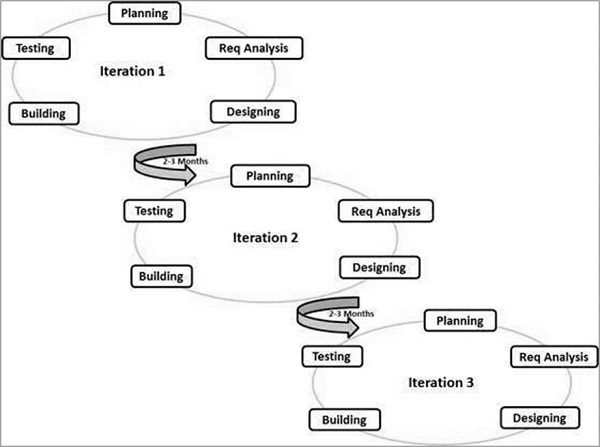
\includegraphics[width=9cm]{agile.jpg}
    \end{center}
    \caption{Agile model}
    \label{fig:agile}
\end{figure}

The philosophy of Agile is that every project needs to be handled differently and the existing methods
need to be tailored to best suit the project requirements. To deliver specific features for a 
release the tasks are divided into time boxes (small time frames).

Agile uses an iterative approach and  working software build is delivered after each iteration. 
Each build is incremental in terms of features; the final build holds all the features required 
by the customer. Refer to figure \ref{fig:agile}.

Following are the Agile Manifesto principles:

\begin{itemize}
    \item \textbf{Working software:} The best means of communication with the customers to understand
    their requirements is by using demo working software, instead of just depending on documentation.
     
    \item \textbf{Customer collaboration:} Continuous customer interaction is very important to get proper
    requirements ,as the requirements cannot be gathered completely in the beginning of the project due 
    to various factors.

    \item \textbf{Responding to change:} The focus is on quick response to changes and 
    continuous development in agile development.
\end{itemize}

\subsection{Agile v/s traditional SDLC Models}

Traditional SDLC models are based on a predictive approach. Teams in traditional SDLC models 
usually work with detailed planning and have a complete view of the exact tasks and features 
to be delivered during the product life cycle. These models entirely depend on the requirement 
analysis and planning done in the beginning of the product life cycle. Any changes to be done go 
through a strict change control management and prioritization.

On the other hand Agile uses an adaptive approach where there is no detailed planning and clarity
of what features need to be developed in future. The team adapts to the  changing product requirements 
dynamically. Agile has minimum failure as the product is tested frequently through the release iterations.

The backbone of agile methodology is customer interaction  and open communication with minimum 
documentation are the typical features of agile. The teams in agile methodology are in close collaboration 
with each other and are often based in the same geographical location.

\subsection{Pros}
\begin{itemize}
    \item Agile is a very realistic approach to software development.
    \item Functionality can be developed, rapidly demonstrated and promotes teamwork and cross training. 
    \item Resource requirements are minimum.
    \item It delivers early partial working solutions and is suitable for fixed or changing requirements.
    \item Good model for environments that change steadily.
    \item Minimal rules, documentation easily employed and little or no planning required.
    \item Gives flexibility to developers.
\end{itemize}

\subsection{Cons}
\begin{itemize}
    \item Not suitable for handling complex dependencies and more risk of sustainability, maintainability and extensibility.
    \item Strict delivery management dictates the scope, functionality to be delivered, and adjustments to meet the deadlines.
    \item Depends heavily on customer interaction, so if the customer is not clear, the team can be driven in the wrong direction.
    \item Has a very high individual dependency, since there is minimum documentation generated and transfer of technology to new 
    team members may be quite challenging due to lack of documentation.
\end{itemize}

\section{CI/CD pipeline}
A CI/CD pipeline automates you software delivery process. The pipeline builds codes, runs test (CI),
and safely deploys a new version of the application (CD).

\subsection{CI and CD}
CI stands for Continuous Integration. It is a development process in which the developers merge
their code changes multiple times a day in a central repository. With CI, each change in code 
triggers an automated build and test sequence.

CD stands for Continuous Delivery which on top of continuous integration adds the practice of 
automating the entire software release process. CD includes infrastructure provisioning and deployment 
which may be manual and consists of multiple stages.

\subsection{Elements of CI/CD}

\begin{figure}[h!]
    \begin{center}
        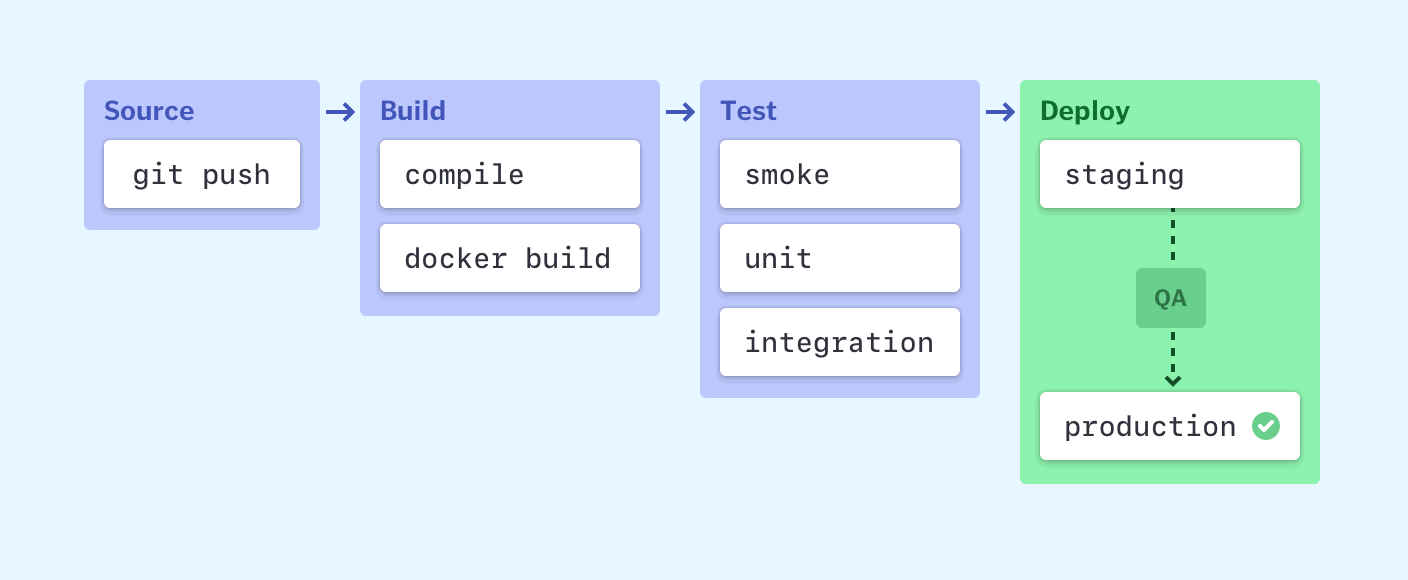
\includegraphics[width=15cm]{cicd.png}
    \end{center}
    \caption{Elements of CI/CD}
    \label{fig:cicd}
\end{figure}

\subsubsection{Source Stage}
Source repository triggers a pipeline run. A notification is triggered to the CI/CD tool 
which runs the corresponding pipeline if there is a change in code. 

\subsubsection{Build Stage}
To build a runnable instance of our product that we can potentially ship to our end users we combine 
the source code and its dependencies . Programs written in languages such as Java, C/C++, or Go need 
to be compiled, whereas Ruby, Python and JavaScript programs work without this step.

Regardless of the language, cloud-native software is typically deployed with Docker, in which case this 
stage of the CI/CD pipeline builds the Docker containers.

There are fundamental problems in the project's configuration if the project fails to pass the build 
stage, and it’s best to address the problems immediately.

\subsubsection{Test Stage}
We run automated tests to validate our code and the behaviour of our product. This stage acts as a safety
net that does not allow the bugs to reach the end-users.

This stage can last from seconds to  hours depending on the complexity of the project.

Failure in this stage shows the errors in the code that developers didn't foresee when writing the code.

\subsubsection{Deploy Stage}
Once the runnable instance of the code has passed all the test stages, it is ready to deploy. There are 
multiple deploy environments for example “beta” environment for the product team and “production” 
environment for end-users.

Teams that have embraced the Agile model of development guided by tests and real-time monitoring usually 
deploy work-in-progress manually to a beta environment for additional manual testing and review, and 
automatically deploy approved changes from the master branch to production.

% High Level Diagram showing microservices.
\section{High Level Systems}

\begin{figure}
    \centering
    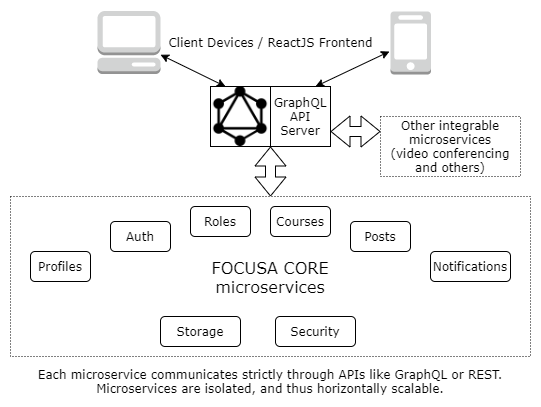
\includegraphics[width=12cm]{High Level.png}
    \caption{High Level Diagram illustrating all microservices of our application.}
    \label{fig:highlevel}
\end{figure}

Microservices, also known as the microservice architecture, is an architectural style that structures an 
application as a collection of services that are
\begin{itemize}
    \item Highly maintainable and testable
    \item Loosely coupled
    \item Independently deployable
\end{itemize}

The microservice architecture enables the rapid, frequent and reliable delivery of large, complex applications.
The benefits of decomposing an application into different, smaller services are:
\begin{itemize}
    \item \textbf{Modularity:} This makes the application easier to understand, develop, test, and 
    become more resilient to architecture erosion.
    \item \textbf{Scalability:} Since microservices are implemented and deployed independently of 
    each other, i.e. they run within independent processes, they can be monitored and scaled independently.
    \item \textbf{Integration of heterogeneous and legacy systems:} Microservices are considered as a 
    viable mean for modernizing existing monolithic software application.
    \item \textbf{Distributed development:} It parallelizes development by enabling small autonomous teams to
    develop, deploy and scale their respective services independently. It also allows the architecture of 
    an individual service to emerge through continuous refactoring.
\end{itemize}

Our project FOCUSA, will include the following microservices, refer to figure \ref{fig:highlevel}:
\begin{itemize}
    \item \textbf{Auth:} performs the authentication process based on a username and password, and returns refresh cookies with a JWT.
    \item \textbf{Roles:}  returns the roles that a user belongs to. It depicts the different roles that different admins perform.
    \item \textbf{Profiles:} Each user has a unique profile, containing details like the user display picture, username, and the various courses the user has subscribed to.
    \item \textbf{Courses:}  returns the details of the courses which includes the course title and the different users subscribed to the course, as well as a provision for new users to subscribe to the course. Only users with certain roles can moderate their respective courses.
    \item \textbf{Posts:} refers to posts posted by the course moderators. The moderators are able to perform CRUD operations on these posts
    \item \textbf{Notifications:}  pushes notifications to the user devices and also monitors the database for changes.
\end{itemize}

\subsection{Using GraphQL with the Microservices}

We make  use of a single GraphQL Schema as an API Gateway to all the microservices together, 
integrating it under a single application. This enables integration of data from the different services.

One of the main benefits of having everything behind a single endpoint, is that data can be routed more 
effectively than if each request had its own service. 

The microservices handle the business logic themselves, while the GraphQL platform interacts with the 
clients to process the queries by consulting the services using REST API, thus allowing for easier isolation 
and horizontal scaling.

% Activity Diagram
\section{Activity Diagram}

\begin{figure}[h!]
    \begin{center}
        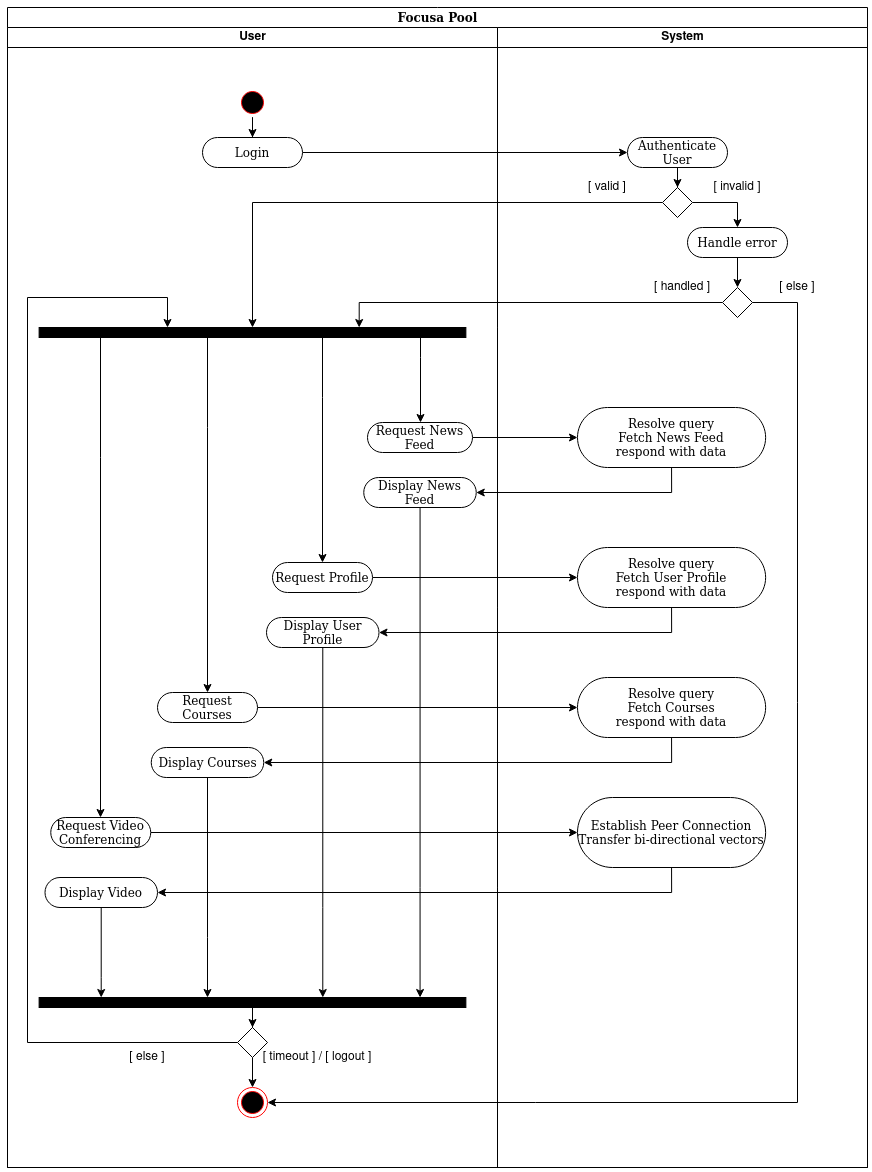
\includegraphics[width=15cm]{activity.png}
    \end{center}
    \caption{Activity Diagram}
    \label{fig:activity}
\end{figure}

Refer to figure \ref{fig:activity}. The user logs in to the app by putting in the valid credentials.
The credentials put in by the user are validated by the system through the authentication mechanism on the server.
If the credentials are found to be incorrect, the system runs the error handler to address the error occurred.
If the user still is not able to produce the correct credentials, the process ends and the user is not allowed to use the app.

If the user has been validated and is found to be genuine, is directed to the home/main page of the app where he can choose to request for the News Feed, User Profile, Courses or launch video conferencing.
All these requests can be made through the navigation panel provided in the app and are accessed as parallel activities.

Once the user requests for a service, the request is sent to the system as a query which is then resolved by the GraphQL to extract the specific requested data from the backend and the response returned is then displayed to the user in structured format.

If the user requests to launch the video conferencing, the system estblishes a peer to peer connection with the requested user system, asks the user to grant access to the camera and audio and starts transfering bi-directional vectors as the secure connection is established.
These bi-directional vectors are worked upon by the algorithm used to reduce the bandwidth usage and the output is displayed in the form of video.

If the user decides to log out of the app, it can be accomplished via the corresponding UI component and as a result all the parallel activities combine to close and the user is logged out of the app safely .
The user is also logged out of the app the session times out.

% Schema diagram.
\section{Database Schema Diagram}

\begin{figure}[h!]
    \centering
    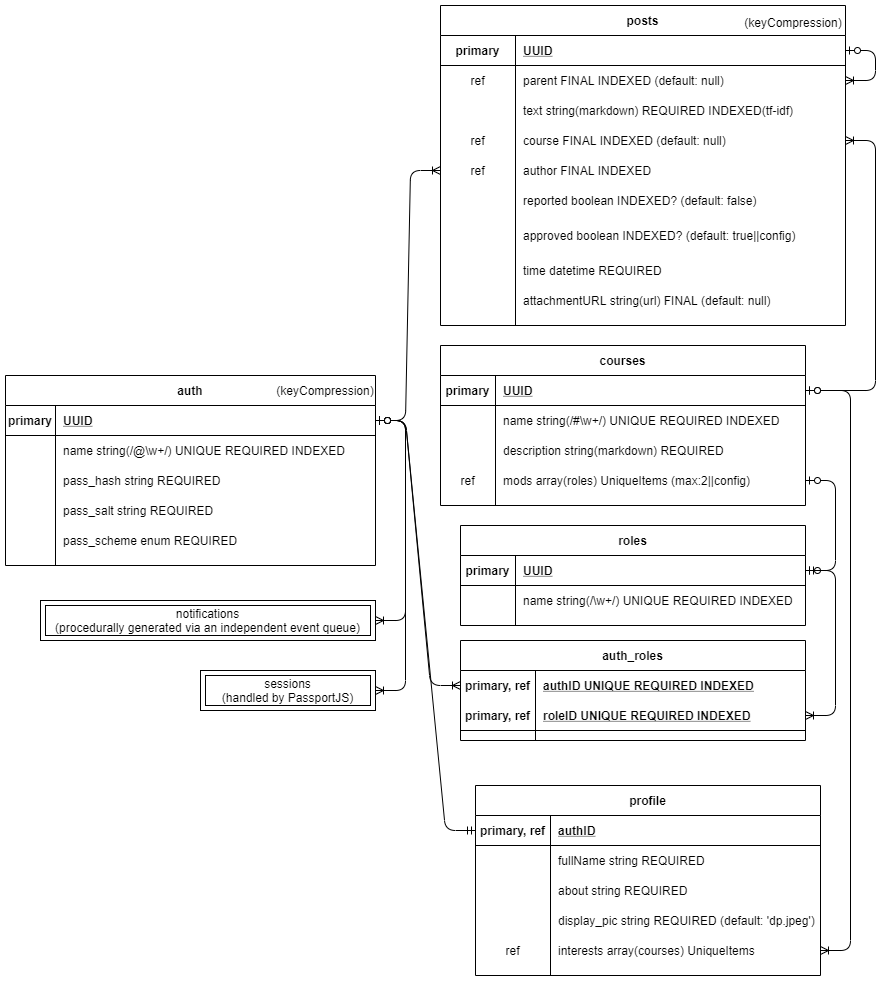
\includegraphics[width=15cm]{db-schema.png}
    \caption{The Database Schema Diagram illustrates the Collections and document schemas, along with references.}
\end{figure}

% Sequence Diagram.
\section{Sequence Diagram}

\begin{figure}[h!]
    \begin{center}
        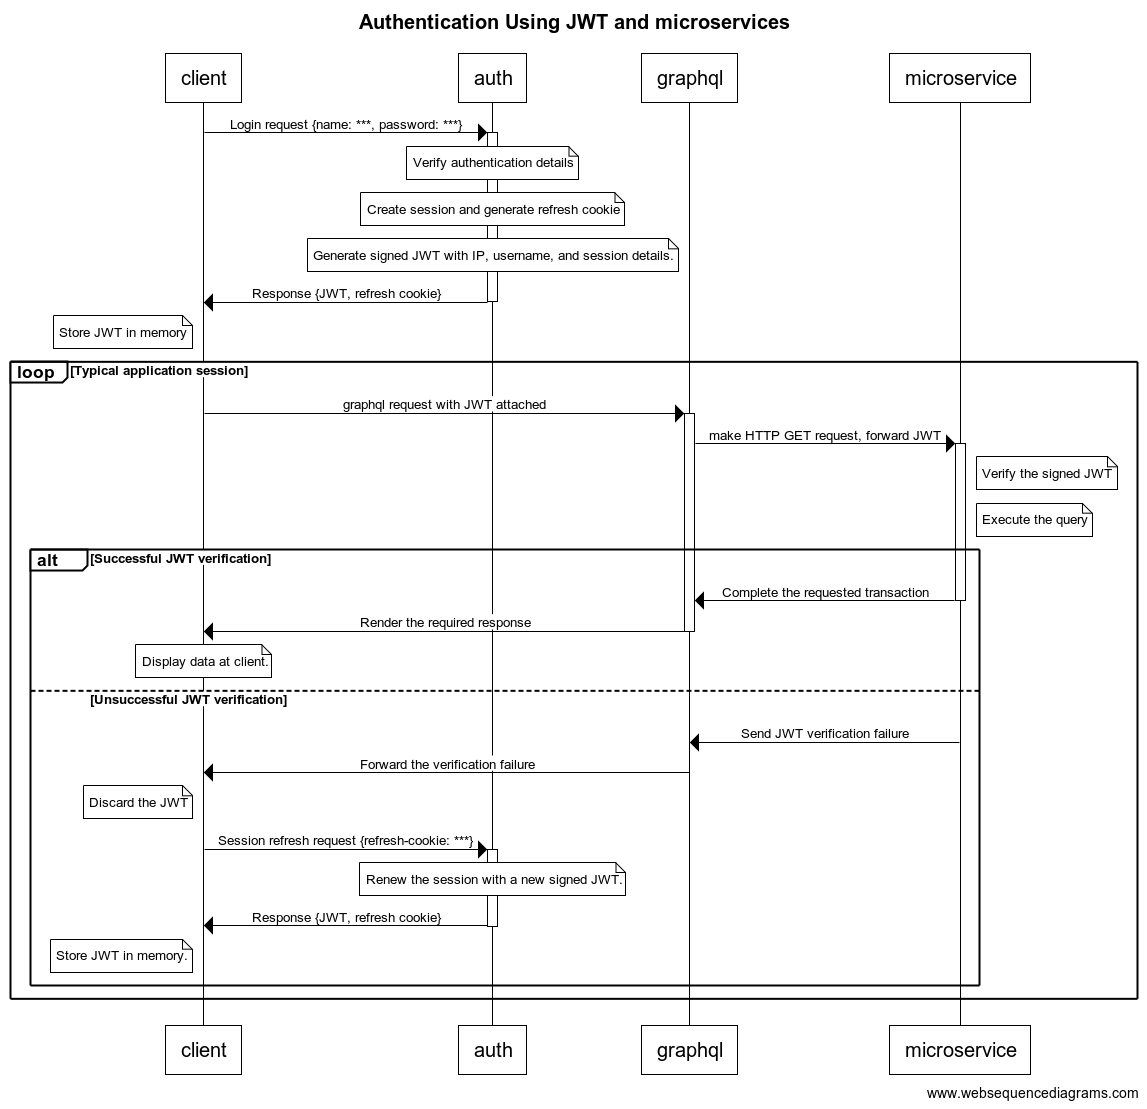
\includegraphics[width=15cm]{sequence.png}
    \end{center}
    \caption{Authentication Sequence Diagram. This diagram illustrates four actors: client, auth, GraphQL, microservice.}
    \label{fig:sequence}
\end{figure}

Refer to figure \ref{fig:sequence}.
The client sends a request to login to the auth microservice along with the credentials ie; name, password.
On receiving the credentials the auth verifies the authentication details, finding it correct, creates a session and generates a refresh cookie.
Auth also generates a signed JWT(JSON Web Token) conatining the IP, username and session details of the client.

This JWT is stored in the client memory and acts as an ID card which can be used by 
the client to directly work with the GraphQL and microservices without the need of 
the authentication with the auth time and again.
The JWT along with the refresh cookie is sent as a response to the user by the auth.

The client can now communicate with GraphQL by showing the JWT and request for data.
The GraphQL makes an HTTP GET request and forwards JWT to the requested microservice.
The microservice verifies the signed JWT received from the GraphQL and if found valid 
executes the query and returns response data to the GraphQL.
Grapql converts the recevied response into a required format and sends it to the client.
This is incase of successful JWT verification

Incase the microservice finds the JWT to be invalid it sends a failure response to the 
GraphQL wich inturn returns the failure response to the client.
The client now needs to request the auth for a session refresh upon which the auth 
returns a new signed JWT along with the refresh cookie.

On refresh the JWT gets deleted from memory and is no longer valid. The client needs 
to request for a session renew and a new signed JWT.
On logout the JWT is simply discarded by deleting the object from memory. 

% Neural Network architecture diagram.

\chapter{Implementation}

% Just added a stub.
% TODO: Complete and fill up the implementation chapter!

% Include experiments and observations from the neural network experiment.
% Also include the process of creating microservices: 1. CRUD. 2. REST. 3. GraphQL.
% Also include the methods of test cases performed.
% Also include the Kubernetes and other deployment stuff.
% Talk about how we are implementing the couchDB distributed DBs.
\chapter{\centering Conclusion}

\section{Discussion}
Distributed databases like CouchDB operate with eventual consistency. The CAP theorem proves beyond doubt that it is close to impossible 
to actually achieve consistency, availability and partition tolerance simultaneously, unless we manage to build successful quantum communication.

Microservices are containerized and isolated, allowing for loosely coupled, highly scalable and secure architectures. The slight learning curve required 
to use message passing over shared memory and APIs is large, but beneficial, since message passing can be used when building any application, even if it is 
not a microservice application.

Microservices by themselves do not manage data storage, but only processing and interfacing. Thus, the use of an efficient, distributed and easy 
to synchronise database like CouchDB, and file server like IPFS allows for efficient scaling and replication, along with support for sharding. This means that the system can 
easily implement a RAID-style disk management, but at the application layer, with faster and easier scaling.

Cross-platform tools like React Native for building a mobile app frontend really simplify the development of User Interfaces. Problems still exist when 
trying cross-compatibility features, and algorithms mostly perform worse than a direct native code. With Expo SDK, support for multiple platforms, including 
the web (through Expo Snack) make React Native a go-to solution for building UIs.

Finally, GANs (Generative Adversarial Networks) perform better than VAEs (Variational Auto-Encoders) for video conferencing codecs. 
Neural networks designed solely for encoding tasks perform poorly because of the way they are trained. Most loss functions like MSE tend to give an average probability 
distribution instead of a reconstruction. GANs perform much better at generative and reconstructive tasks due to their min-max training algorithm, and are well-suited for codecs.

The only bottleneck for neural network codecs is currently the massive amount of computation resources required for smooth operation. This is mainly because 
most research models are not knowledge distilled. Knowledge distillation can help ease the computation requirements, reduce the model sizes and still stay at 
par with the original model's performance. Knowledge distillation will surely bring in the commercialization of neural network codecs. NVIDIA Maxine may have tried neural 
network optimisations and cloud processing, but it defeats the purpose of offline functionailty and overall reduced network bandwidth usage.

\section{Conclusion}
Our project delivered the following:
\begin{itemize}
    \item A Learning Management System built on an offline-first supported architecture, using file and post caching.
    \item A GraphQL API backend, with greatly reduced network requirements. It can operate independent of a reliable 
    and high bandwidth connection.
    \item A truly peer to peer notification service which operates using a pull notification PubSub architecture, 
    transferring data using binary streams and protocol buffers.
    \item Multiple video conferencing implementations, each operating on different strategies, 
    and working with various open source technologies.
    \item A Proof of Concept illustrating an implementation of a neural network as a realtime video codec for video conferencing.
\end{itemize}

Our Proof of Concept successfully used the pre-trained First Order Motion Model (FOMM) to illustrate reduces
network bandwidth usage. It also showcased the possibility of a neural network being potentially used as a codec 
for video conferencing whenever computers are capable enough.

\section{Future Scope}
In hindsight, our project has large scope. The team feels fulfilled for having arrived at the current state of the project. 
However, we do not want to stop here. There are a lot of things we would like to do in the future, and eventually convert this 
project into a commercially viable product. The project is far from over.

The first major requirement would be to actually train a distilled neural network as a video conferencing codec, and commercially 
integrate it in to an existing video conferencing application, like Jitsi. The major bottlenecks would include obtaining a video training dataset 
(the one we needed was licensed and closed behind a paywall, while also being around 300GB in size, and needed manual web scraping), and also a very powerful computer to train multiple networks in parallel. 
Ultimately, distilled networks will operate in a highly optimised manner, but require massive amounts of training to do so.

Finally, we noticed that the current industrial standards for building nodeJS microservice applications do not have the level of transparency and 
distributed nature as would be desired by us. While serverless architectures do exist, they still suffer from various bottlenecks like ephemeral 
data storage. Libp2p is a standard library created by the IPFS team which allows for cross-protocol communication in a truly distributed manner, 
allowing for dynamic transfers of location, concurrency, replication, and migration. Libp2p however does not have an official RPC implementation 
which can be publicly used. We would like to venture into contributing this feature to libp2p as it would really help in commercial DevOps.

GraphQL API allows for very efficient querying of data using resolvers, with support for fine-grained interospection and optimizations like caching 
on both the server and client. Using GraphQL over a new protocol stack like the upcoming HTTP/3 (QUIC protocol), or simply using protocol buffers over 
HTTP. These steps alone can reduce the internet bandwidth requirements by almost 60 percent. We believe that using a truly distributed architecture at the 
server side, and efficient data transfer to client side can double our application performance and experience.

\bibliographystyle{plain}
\bibliography{chapters/references}
\pdfbookmark{\bibname}{Bibliography}
\end{document}